\chapter{Arduino}
\label{chap:arduino}

%%%%%%%%%%%%%%%%%%%%%%%%%%%%%%%%%%%%%%%%%%%%%%%%%%%%%%%%%%%%%%%%%%%%%%%%%%%%%%%%
% Objetivo: Exponer la plataforma Arduino                                      %
%%%%%%%%%%%%%%%%%%%%%%%%%%%%%%%%%%%%%%%%%%%%%%%%%%%%%%%%%%%%%%%%%%%%%%%%%%%%%%%%

\lettrine{A}{rduino} \cite{WikipediaArduino} é unha plataforma de hardware e
software libre, baseada nunha placa cun microcontrolador e un entorno de
desenvolvemento (IDE), deseñada para facilitar o uso da electrónica en
proxectos multidisciplinares. \\

O hardware consiste nunha placa cun microcontrolador \textit{Atmel AVR} e
portos de entrada/saída. Os microcontroladores máis usados son o
\textit{Atmega168}, \textit{Atmega328}, \textit{Atmega1280}, \textit{ATmega8}
pola súa sinxeleza e baixo custo que permiten o desenvolvemento de múltiples
deseños. Doutra banda o software consiste nun contorno de desenvolvemento que
implementa a linguaxe de programación con \textit{Processing} e \textit{Wiring}
e o cargador de arrinque (\textit{boot loader}) que corre na placa. \\

Arduino pódese utilizar para desenvolver obxectos interactivos autónomos ou
pode ser conectado a software do computador (por exemplo:
\textit{Macromedia Flash}, \textit{Processing}, \textit{Max/MSP},
\textit{Pure Data}). As placas pódense montar a man ou adquirirse. O contorno
de desenvolvemento integrado libre pódese descargar gratuitamente. \\

Ó ser open-hardware, tanto o seu deseño como a súa distribución é libre.
É dicir, pode utilizarse libremente para o desenvolvemento de calquera tipo de
proxecto sen adquirir ningunha licenza. \\

O proxecto Arduino recibiu unha mención honorífica na categoría de
\textit{Comunidades Dixitais} no \textit{Prix Ars Electronica} de 2006.

\section{Historia}

En 2005, en Ivrea, Italia no \textit{Interaction Design Institute} (fundado por
\textit{Olivetti} e \textit{Telecom Italia}), iniciouse o proxecto para facer
un dispositivo controlador programable construído por estudiantes de deseño
para proxectos interactivos de baixo custe para sistemas de prototipado. Os
fundadores Massimo Banzi e David Cuartielles chamaron ó proxecto despois
\textit{Arduin de Ivrea}, tomando o nome dun bar que o tomara a súa vez de
\textit{Arduino d'Ivrea}, primeiro rei de Italia en 1002. \textit{Arduino} é
tamén un nome de home, que en italiano significa \textit{amigo valente}. \\

O proxecto Arduino é unha plataforma de código aberto (IDE) para plataformas
(GNU/Linux, Mac e Windows). O artista colombiano e programador
Hernando Barragán creouno como tese no
\textit{Interaction Design Institute Ivrea} baixo a supervisión de
Massimo Banzi e Casey Reas. \textit{Wiring} baséase en \textit{Processing} e o
seu entorno de desenvolvemento integrado, que fora creado por Casey Reas e Ben
Fry. \\

Grazas á base de software común, dos creadores do proxecto para a comunidade
Arduino foi posible desenvolver programas para conectar con este hardware máis
ou menos calquera obxecto electrónico, ordenador, sensores, pantallas e
actuadores. Despois de anos de experimentación, agora é posible beneficiarse
dunha ampla base de datos e información.

\section{Instalación}

\begin{figure}[htbp]
 \centering
 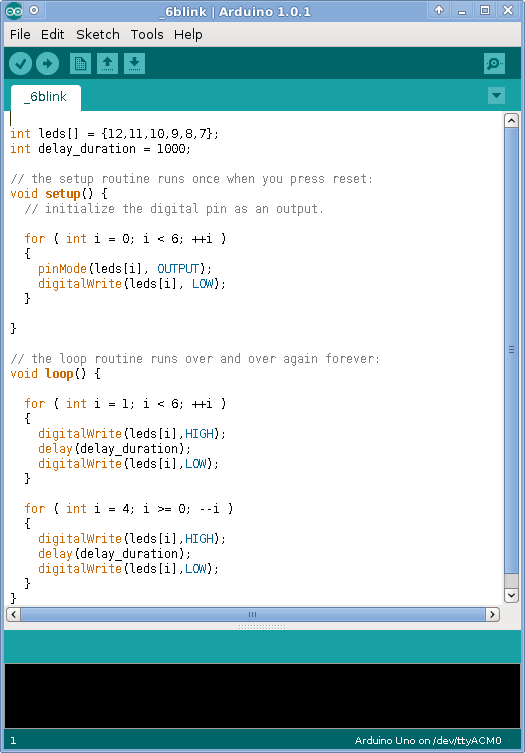
\includegraphics[scale=0.3,keepaspectratio=true]{./imagenes/arduino-sketch.png}
 % arduino-sketch.png: 525x753 pixel, 72dpi, 18.52x26.56 cm, bb=0 0 525 753
 \caption{IDE Arduino}
 \label{figura:ArduinoSketch}
\end{figure}

 \subsection{Windows}

 Para a instalación da placa Arduino no sistema operativo Windows convén seguir
 os seguintes pasos. \\

 Coa placa desconectada:

 \begin{itemize}
  \item Descargar e instalar o \textit{Java Runtime Enviroment} (J2RE).
  \item Descargar a última versión do \textit{IDE Arduino}.
 \end{itemize}

 É recomendable descomprimir o ficheiro no directorio raíz (C:\textbackslash)
 mantendo a estrutura orixinal. \\
 
 Entre todos os cartafoles creados no directorio Arduino convén destacar as
 seguintes: \\

 \begin{lstlisting}[language=bash,frame=single]
  c:\arduino-0012\hardware\bootloader
 \end{lstlisting}

 Esta contén o software necesario para cargar o firmware no chip
 \textit{Atmega168}, para traballar con Arduino. Só se utiliza en caso
 empregar placas artesanais. \\

 \begin{lstlisting}[language=bash,frame=single]
  c:\arduino-0012\drivers
 \end{lstlisting}

 Contén os drivers necesarios para o funcionamento da placa Arduino cun PC con
 S.O. Windows: \textit{FTDI USB Drivers}. \\

 Para instalar estes drivers, agora si, conectar  a placa USB. Abrirase
 automaticamente o asistente de Windows para novo hardware atopado.

 \begin{enumerate}
  \item Seleccionar ``Non polo momento'' e premer en ``Seguinte''.
  \item Seleccionar
        ``Instalar desde unha lista ou localización específica (avanzado)'' e
        premer en ``Seguinte''.
  \item ``Buscar o controlador máis adecuado nestas localizacións'', premer en
        ``Examinar''. Seleccionar o cartafol onde se descomprimira o driver e
          premer ``Seguinte''.
 \end{enumerate}

 Se non houbo ningún problema o driver da placa estará instalado. \\

 Agora executamos o ficheiro \textit{Arduino.exe} para abrir a interface. Aquí
 configuramos o porto USB onde temos conectada a placa para empezar a
 traballar.

 \subsection{GNU/Linux}

 Para instalar Arduino nun sistema GNU/Linux necesitamos os seguintes programas
 para resolver as dependencias:

 \begin{itemize}
  \item Sun Java runtime, \textit{jre}, ou equivalente.
  \item \textit{avr-gcc}, compilador para a familia de microcontroladores AVR de
        Atmel.
  \item \textit{avr-libc}, libc do compilador avr-gcc.
 \end{itemize}

 Para instalalos, podemos utilizar o xestor de paquetes ou a terminal de
 comandos: \\

 \begin{lstlisting}[language=bash,frame=single]
  apt-get install sun-java5-jre gcc-avr avr-libc
 \end{lstlisting}

 Nalgunhas distribucións convén desinstalar, se non é necesario, o paquete
 \textit{brltty}. Este encárgase de permitir o acceso á terminal para persoas
 cegas a través dun dispositivo especial en Braille. \\

 \begin{lstlisting}[language=bash,frame=single]
  killall brltty
  apt-get remove brltty
 \end{lstlisting}

 Os dous síntomas deste problema son:

 \begin{itemize}
  \item Non aparece a opción \textit{/dev/tty/USB0} no menú
        \textit{Tools, Serial Port}.
  \item Se se observa o LED Rx da placa Arduino, e este se ilumina de 3 a 5
        veces cada 5 ou 6 segundos.
 \end{itemize}

 Por último, descargamos o framework de Arduino. Descomprimímolo no cartafol
 desexado e executámolo: \\

 \begin{lstlisting}[language=bash,frame=single]
  ./arduino
 \end{lstlisting}

 Se todo foi ben xa o teremos en funcionamento.

\section{Hardware}

 \subsection{Placas Arduino}

 Unha placa Arduino consta de un microcontrolador de 8-bit \textit{Atmel AVR}
 con compoñentes complementarios para facilitar a programación e a
 incorporación noutros deseños. Un aspecto importante de Arduino é a forma
 estándar na que dispóñense os conectores, permitindo que a placa da CPU poida
 ser conectada a unha variedade de módulos intercambiables adicionais coñecidos
 como \textit{shields}. Algúns comunícanse cos shields da placa Arduino
 directamente cos diferentes pins, pero moitos shields son individualmente
 direccionables a través dun bus I2C de serie, o que permite que moitos shields
 poidan apílarse e empregarse en paralelo. As placas Arduino oficias empregan a
 serie de circuítos integrados \textit{megaAVR}, específicamente o
 \textit{ATmega8}, \textit{ATmega168}, \textit{ATmega328}, \textit{ATmega1280}
 e \textit{ATmega2560}. Un feixe doutros procesadores compatibles foron
 empregados por Arduino. A maioría das placas inclúen un regulador lineal de 5
 voltios e un oscilador de 16 MHz de reloxo (ou oscilador de cuarzo nalgunhas
 variantes), aínda que algúns deseños, tales como o \textit{LilyPad} son a 8
 MHz e prescinde do regulador de tensión integrado na placa, debido a
 restricións determinadas polo deseño. Un microcontrolador Arduino está tamén
 pre-programado con un xestor de arranque que simplifica a carga de programas
 na memoria flash do chip, en comparación con outros dispositivos que
 normalmente necesitan un programador externo ou hardware adicional. \\

 A nivel conceptual, cando se utiliza a pila de software de Arduino, todas as
 placas se programan a través dunha conexión \textit{RS-232}, pero a forma en
 que isto se fai varía segundo a versión do hardware. As placas serie Arduino
 conteñen un circuíto inversor simple para converter entre o nivel
 \textit{RS-232} e os sinais de nivel TTL. As actuais placas Arduino
 prográmanse a través de portos USB, implementado a través dun circuíto
 \textit{FT232 FTDI}. Algunhas variantes, como o \textit{Mini Arduino} e o non
 oficial \textit{Boarduino}, empregan un cable de datos USB, \textit{Bluetooth}
 ou outros métodos. Cando se emprega con ferramentas para microcontroladores
 tradicionais en vez do \textit{IDE Arduino}, emprégase o estándar de
 programación \textit{AVR ISP}. \\

 A maioría das placa Arduino conectan os pins do microcontrolador como
 entradas/saídas para o seu uso por otros circuítos. O \textit{Diecimila},
 \textit{Duemilanove}, e o actual \textit{Uno} proporcionan 14 pins E/S
 dixitais, seis dos cales poden producir pulsos de ancho variable, e seis
 entradas analóxicas (PWM). Estes pins atópanse na parte superior do taboleiro,
 a través de conectores femia de 0,1 polgadas. Tamén están dispoñibles
 comercialmente varias shields oficiais de tipo Plug-in.

 \subsection{Linguaxe de programación Arduino}

 A plataforma Arduino prográmase mediante o uso dunha linguaxe propia baseada
 na popular linguaxe de programación de alto nivel \textit{Processing}. Con
 todo, é posible utilizar outras linguaxes de programación e aplicacións
 populares en Arduino. Algúns exemplos son:

 \begin{itemize}
  \item Java
  \item Flash (mediante ActionScript)
  \item Processing
  \item Pure Data
  \item MaxMSP (contorna gráfica de programación para aplicacións musicais, de audio e multimedia)
  \item VVVV (síntese de vídeo en tempo real)
  \item Adobe Director
  \item Python
  \item Ruby
  \item C
  \item C++ (mediante libSerial ou en Windows)
  \item C\#
  \item Cocoa/Objective-C (para Mac OS X)
  \item GNU/Linux TTY (terminais de GNU/Linux)
  \item 3DVIA Virtools (aplicacións interactivas e de tempo real)
  \item SuperCollider (síntese de audio en tempo real)
  \item Instant Reality (X3D)
  \item Liberlab (software de medición e experimentación)
  \item BlitzMax (con acceso restrinxido)
  \item Squeak (implementación libre de Smalltalk)
  \item Mathematica
  \item Matlab
  \item Minibloq (Contorna gráfica de programación, corre tamén en OLPC)
  \item Isadora (Interactividade audiovisual en tempo real)
  \item Perl
  \item Visual Basic .NET
  \item VBScript
  \item Gambas
 \end{itemize}

 Isto é posible debido a que Arduino se comunica mediante a transmisión de
 datos en formato serie que é algo que a maioría das linguaxes anteriormente
 citadas soportan. Para os que non soportan o formato serie de forma nativa, é
 posible utilizar software intermediario que traduza as mensaxes enviadas por
 ambas as partes para permitir unha comunicación fluída. É bastante interesante
 ter a posibilidade de interactuar Arduino mediante esta gran variedade de
 sistemas e linguaxes posto que dependendo de cales sexan as necesidades do
 problema que imos resolver poderemos aproveitarnos da gran compatibilidade de
 comunicación que ofrece.

  \subsubsection{Funcións básicas e operadores}

  Arduino esta baseado en C e soporta todas as funcións do estándar C e
  algunhas de C++. A continuación móstrase un resumo con tódalas estruturas da
  linguaxe Arduino:

   \paragraph{Sintaxe básica}

   \begin{itemize}
    \item Delimitadores: ;, \{\}
    \item Comentarios: //, /* */
    \item Cabeceiras: \#define, \#include
    \item Operadores aritméticos: +, -, *, /, \%
    \item Asignación: =
    \item Operadores de comparación: ==, !=, \verb|<|, \verb|>|, \verb|<|=, \verb|>|=
    \item Operadores Booleanos: \&\&, \texttt{||}, !
    \item Operadores de acceso a punteiros: *, \&
    \item Operadores de bits: \&, |, \verb|^|, \verb|<<|, \verb|>>|
    \item Operadores compostos:
          \begin{itemize}
           \item Incremento/decremento de variables: ++, \verb|--|
           \item Asignación e operación: +=, -=, *=, /=, \&=, \texttt{|=}
          \end{itemize}
   \end{itemize}

   \paragraph{Estruturas de control}

   \begin{itemize}
    \item Condicionais: if, if...else, switch case
    \item Bucles: for, while, do... while
    \item Bifurcaciones e saltos: break, continue, return, goto
   \end{itemize}

   \paragraph{Variables}\mbox{}\\

   En canto ao tratamento das variables tamén comparte un gran parecido coa
   linguaxe C.

   \paragraph{Constantes}

   \begin{itemize}
    \item HIGH / LOW: niveis alto e baixo en pines. Os niveis altos son aqueles
          de 3 voltios ou máis.
    \item INPUT / OUTPUT: entrada ou saída
    \item true / false
   \end{itemize}

   \paragraph{Tipos de datos}

   \begin{itemize}
    \item void
    \item boolean
    \item char
    \item unsigned char
    \item byte
    \item int
    \item unsigned int
    \item word
    \item long
    \item unsigned long
    \item float
    \item double
    \item string
    \item array
   \end{itemize}

   \paragraph{Conversión entre tipos}\mbox{}\\

   Estas funcións reciben como argumento unha variable de calquera tipo e
   devolven unha variable convertida no tipo desexado.

   \begin{itemize}
    \item char()
    \item byte()
    \item int()
    \item word()
    \item long()
    \item float()
   \end{itemize}

   \paragraph{Cualificadores e ámbito das variables}

   \begin{itemize}
    \item static
    \item volatile
    \item const
   \end{itemize}

   \paragraph{Utilidades}

   \begin{itemize}
    \item sizeof()
   \end{itemize}

   \paragraph{Funcións básicas}\mbox{}\\

   En canto ás funcións básicas da linguaxe atopámonos coas seguintes:

    \subparagraph{E/S Dixital}

    \begin{itemize}
     \item pinMode(pin, modo)
     \item digitalWrite(pin, valor)
     \item int digitalRead(pin)
    \end{itemize}

    \subparagraph{E/S Analóxica}

    \begin{itemize}
     \item analogReference(tipo)
     \item int analogRead(pin)
     \item analogWrite(pin, valor)
    \end{itemize}

    \subparagraph{E/S Avanzada}

    \begin{itemize}
     \item shiftOut(dataPin, clockPin, bitOrder, valor)
     \item unsigned long pulseIn(pin, valor)
    \end{itemize}

    \subparagraph{Tempo}

    \begin{itemize}
     \item unsigned long millis()
     \item unsigned long micros()
     \item delay(ms)
     \item delayMicroseconds(microsegundos)
    \end{itemize}

    \subparagraph{Matemáticas}

    \begin{itemize}
     \item min(x, e)
     \item max(x, e)
     \item abs(x)
     \item constrain(x, a, b)
     \item map(valor, fromLow, fromHigh, toLow, toHigh)
     \item pow(base, expoñente)
     \item sqrt(x)
    \end{itemize}

    \subparagraph{Trigonometría}

    \begin{itemize}
     \item sin(rad)
     \item cos(rad)
     \item tan(rad)
    \end{itemize}

    \subparagraph{Números aleatorios}

    \begin{itemize}
     \item randomSeed(semente)
     \item long random(máx)
     \item long random(mín, máx)
    \end{itemize}

    \subparagraph{Bits e Bytes}

    \begin{itemize}
     \item lowByte()
     \item highByte()
     \item bitRead()
     \item bitWrite()
     \item bitSet()
     \item bitClear()
     \item bit()
    \end{itemize}

    \subparagraph{Interrupcións externas}

    \begin{itemize}
     \item attachInterrupt(interrupción, función, modo)
     \item detachInterrupt(interrupción)
    \end{itemize}

    \subparagraph{Interrupcións}

    \begin{itemize}
     \item interrupts()
     \item noInterrupts()
    \end{itemize}

    \subparagraph{Comunicación por porto serie}\mbox{}\\

    As funcións de manexo do porto serie deben ir precedidas de ``Serial.''
    aínda que non necesitan ningunha declaración na cabeceira do programa. Por
    isto se consideran funcións base da linguaxe.

    \begin{itemize}
     \item begin()
     \item available()
     \item read()
     \item flush()
     \item print()
     \item println()
     \item write()
    \end{itemize}

    \subparagraph{Manipulación de portos}\mbox{}\\

    Os rexistros de portos permiten a manipulación a máis baixo nivel e de
    forma mais rápida dos pines de E/S do microcontrolador das placas Arduino.
    Os pines das placas Arduino están repartidos entre os rexistros B(0-7),
    C (analóxicos) e D(8-13). Mediante as seguintes variables podemos ver e
    modificar o seu estado:

    \begin{itemize}
     \item DDR[B/C/D]: Data Direction Register (ou dirección do rexistro de
           datos) do porto B, C ó D. Serve para especificar que pines queremos
           usar como de entrada e cales de saída. Variable de
           lectura/escritura.
     \item PORT[B/C/D]: Data Register (ou rexistro de datos) do porto B, C ó D.
           Variable de lectura/escritura.
     \item PIN[B/C/D]: Input Pins Register (ou rexistro de pines de entrada) do
           porto B, C ó D. Variable de só lectura.
    \end{itemize}

    Por exemplo, para especificar que queremos utilizar os pines 1 a 7 como
    saídas e o 0 como entrada, bastaría utilizar a seguinte asignación: \\

    \begin{lstlisting}[language=C++,frame=single]
     DDRD = B11111110;
    \end{lstlisting}

   \paragraph{A.V.R. Libc}

   Os programas compilados con Arduino enlázanse contra \textit{AVR Libc} polo
   que teñen acceso a algunhas das súas funcións. \textit{AVR Libc} é un
   proxecto de software libre co obxectivo de proporcionar unha biblioteca C de
   alta calidade para utilizarse co compilador GCC sobre microcontroladores
   \textit{Atmel AVR}. Componse de 3 partes:

   \begin{itemize}
    \item avr-binutils
    \item avr-gcc
    \item avr-libc
   \end{itemize}

   A maioría da linguaxe de programación Arduino está escrita con constantes e
   funcións de AVR e certas funcionalidades só se poden obter facendo uso de
   AVR.

    \subparagraph{Interrupcións}\mbox{}\\

    Para desactivar as interrupcións: \\

    \begin{lstlisting}[language=C++,frame=single]
     cli(); // desactiva as interrupcions globais
    \end{lstlisting}

    Para activalas: \\

    \begin{lstlisting}[language=C++,frame=single]
     \item sei(); // activa as interrupcions
    \end{lstlisting}

    Isto afectará ao temporizador e á comunicación serie. A función
    \textit{delayMicroseconds()} desactiva as interrupcións cando se executa.

    \subparagraph{Temporizadores}\mbox{}\\

    A función \textit{delayMicroseconds()} crea o menor retardo posible da
    linguaxe Arduino que rolda os 2us. \\

    Para retardos mais pequenos débese utilizar a chamada de ensamblador textit{nop}
    (non operación). Cada sentenza \textit{nop} executarase nun ciclo de
    máquina (16 Mhz): uns 62.5ns. Faríase da seguinte maneira: \\

    \begin{lstlisting}[language=C++,frame=single]
     __asm__("nop\n\t");
    \end{lstlisting}

    \subparagraph{Manipulación de portos}\mbox{}\\

    A manipulación de portos con código AVR é mais rápida que utilizar a
    función \textit{digitalWrite()} de Arduino.

    \subparagraph{Establecer bits en variables}\mbox{}\\

    \textit{cbi} e \textit{sbi} son mecanismos estándar (AVR) para establecer
    ou limpar bits en PORT e outras variables. \\

    Será necesario utilizar as seguintes cabeceiras para poder utilizalos: \\

     \begin{lstlisting}[language=C++,frame=single]
      # ifndef cbi
      # define cbi(sfr, bit) (_SFR_BYTE(sfr) &= _BV(bit))
      # endif
      # ifndef sbi
      # define sbi(sfr, bit) (_SFR_BYTE(sfr) |= _BV(bit))
      # endif
     \end{lstlisting}

     Para utilizalas hai que pasarlles como argumento a variable PORT e un pin
     para establecelo ou limpalo. \\

     Grazas a estes pequenos hacks teremos a posibilidade de mellorar os tempos
     de execución de certas tarefas críticas ou daquelas que se repitan moitas
     veces obtendo mellores resultados. Non obstante o código fonte que
     escribamos resultará probablemente menos legible se os utilizamos polo que
     haberá que sopesalo en función das nosas necesidades.

    \paragraph{Primeiro contacto: Ola Mundo en Arduino}\mbox{}\\

    O primeiro paso antes de comprobar que a instalación é correcta e empezar a
    traballar con Arduino é abrir algúns exemplos prácticos que veñen
    dispoñibles co dispositivo. É recomendable abrir o exemplo
    \textit{led\_blink} que atoparemos no menú
    \textit{File, Sketchbook, Examples, led\_blink}. Este código crea unha
    intermitencia por segundo nun led conectado no pin 13. É cuestión de
    comprobar que o código é correcto, para iso, prememos o botón que é un
    triángulo (en forma de \textit{play}) e seguidamente faremos un
    \textit{upload} (que é a frecha cara á dereita) para cargar o programa á
    placa. Se o led empeza a pestanexar, todo estará correcto. \\
   
    Vexamos o código necesario para conseguilo: \\

    \begin{lstlisting}[language=C++,frame=single]
     # define LED_PIN 13

     void setup () {

       // Activamos o pin 13 para saida dixital
       pinMode (LED_PIN, OUTPUT);

     }
 
     // Bucle infinito
     void loop () {
 
       // Acendemos o led enviando un sinal alto
       digitalWrite (LED_PIN, HIGH);
 
       // Esperamos un segundo (1000 ms)
       delay (1000);
 
       // Apagamos o led enviando un sinal baixo
       digitalWrite (LED_PIN, LOW);
 
       // Esperamos un segundo (1000 ms)
       delay (1000);
 
     }
   \end{lstlisting}

   A orde de execución será: primeiro faise unha chamada á función
   \textit{init()} que inicializa o programa, despois execútase a función
   \textit{setup()} que configura diversos parámetros, e por último execútase
   un bucle \textit{while(1)} que chama repetidamente á función \textit{loop}.
   Todo iso execútase dentro de \textit{main()} e podería indicarse
   explicitamente (no caso anterior encárgase o IDE de engadir o código que
   omitiu).

\section{Bibliotecas en Arduino}

Para facer uso dunha biblioteca en \textit{Sketch} (o IDE de Arduino), basta
con facer clic sobre \textit{Import Library} no menú, escoller unha biblioteca
e engadirase o \textit{\#include} correspondente.

\begin{itemize}
 \item Serial: lectura e escritura polo porto serie.
 \item EEPROM: lectura e escritura no almacenamento permanente.
       \begin{itemize}
        \item read()
        \item write()
       \end{itemize}
 \item Ethernet: conexión a Internet mediante \textit{Arduino Ethernet Shield}.
       Pode funcionar como servidor que acepta peticións remotas ou como
       cliente. Permítense até catro conexións simultaneamente.
       \begin{itemize}
        \item Servidor
              \begin{itemize}
               \item Server()
               \item begin()
               \item available()
               \item write()
               \item print()
               \item println()
              \end{itemize}
        \item Cliente
              \begin{itemize}
               \item Client()
               \item connected()
               \item connect()
               \item write()
               \item print()
               \item println()
               \item available()
               \item read()
               \item flush()
               \item stop()
              \end{itemize}
       \end{itemize}
 \item Firmdata: comunicación con aplicacións de computador utilizando o
       protocolo estándar do porto serie.
 \item LiquidCrystal: control de LCDs con chipset \textit{Hitachi HD44780} ou
       compatibles. A biblioteca soporta os modos de 4 e 8 bits.
 \item Servo: control de servo motores. A partir da versión 0017 de Arduino a
       biblioteca soporta até 12 motores na maioría de placas \textit{Arduino}
       e 48 na \textit{Arduino Mega}.
       \begin{itemize}
        \item attach()
        \item write()
        \item writeMicroseconds()
        \item read()
        \item attached()
        \item detach()
       \end{itemize}
 \item O manexo da biblioteca é bastante sinxelo. Mediante
       \textit{attach(número de pin)} engadimos un servo e mediante
       \textit{write} podemos indicar os graos que queremos que teña o motor
       (habitualmente de 0 a 180).
 \item SoftwareSerial: comunicación serie en pines dixitais. Por defecto
       Arduino inclúe comunicación só nos pines 0 e 1 pero grazas a esta
       biblioteca podemos realizar esta comunicación co resto de pines.
 \item Stepper: control de motores paso a paso unipolares ou bipolares.
       \begin{itemize}
        \item Stepper(steps, pin1, pin2)
        \item Stepper(steps, pin1, pin2, pin3, pin4)
        \item setSpeed(rpm)
        \item step(steps)
       \end{itemize}
       O manexo é sinxelo. Basta con iniciar o motor mediante \textit{Stepper}
       indicando os pasos que ten e os pines aos que esta asociado. Indícase a
       velocidade á que queiramos que vire en revolucións por minuto con
       \textit{setSpeed(rpm)} e indícanse os pasos que queremos que avance con
       \textit{step(pasos)}.
 \item Wire: envío e recepción de datos sobre unha rede de dispositivos ou
       sensores mediante \textit{Two Wire Interface} (TWI/I2C). Ademais as
       bibliotecas \textit{Matrix} e \textit{Sprite} de \textit{Wiring} son
       totalmente compatibles con Arduino e serven para manexo de matrices de
       leds. Tamén se ofrece información sobre diversas bibliotecas
       desenvolvidas por contribuidores diversos que permiten realizar moitas
       tarefas.
\end{itemize}

 \subsection{Creación de bibliotecas}

 Ademais das bibliotecas base, as que son compatibles e as que achegaron outras
 persoas temos a posibilidade de escribir nosa propia biblioteca. Isto é moi
 interesante por varias razóns: permite dispor de código que pode reutilizarse
 noutros proxectos de forma cómoda; permítenos manter o código fonte principal
 separado das bibliotecas de forma que sexan mantenibles de forma separada; e a
 organización dos programas construídos é máis clara e elegante. \\

 Vexamos un exemplo da creación dunha biblioteca que envía código
 \textit{Morse}. \\

 Creamos o ficheiro \textit{Morse.h} que inclúe a definición da clase
 \textit{Morse} que ten 3 funcións: un construtor (\textit{Morse()}), unha
 función para enviar 1 punto (\textit{dot()}) e unha función para enviar unha
 raia (\textit{dash()}). A variable \textit{\_pin} permite indicar o pin que
 imos utilizar. \\

 \begin{lstlisting}[language=C++,frame=single]
  /*
 
    Morse.h - Library for flashing Morse code.
 
    Created by David A. Mellis, November 2, 2007.
 
    Released into the public domain.
 
  */

  # ifndef Morse_h
  # define Morse_h
  # include "WProgram.h"
 
  class Morse {
 
    public:
 
      Morse(int pin);
 
      void dot();
 
      void dash();
 
    private:
 
      int _pin;
 
  };
  # endif
 \end{lstlisting}

 Ademais necesitaremos un ficheiro \textit{Morse.cpp} co código das funcións
 declaradas. A continuación móstrase o código: \\

 \begin{lstlisting}[language=C++,frame=single]
  /*
 
    Morse.cpp - Library for flashing Morse code.
 
    Created by David A. Mellis, November 2, 2007.
 
    Released into the public domain.
 
  */

  # include "WProgram.h"
  # include "Morse.h"

  Morse::Morse(int pin) {
 
    pinMode(pin, OUTPUT);
 
    _pin = pin;

  }

  void Morse::dot() {
 
    digitalWrite(_pin, HIGH);
 
    delay(250);
 
    digitalWrite(_pin, LOW);
 
    delay(250);
 
  }

  void Morse::dash() {
 
    digitalWrite(_pin, HIGH);
 
    delay(1000);
 
    digitalWrite(_pin, LOW);
 
    delay(250);
 
  }
 \end{lstlisting}

 E con isto xa poderiamos utilizar a biblioteca mediante o correspondente
 \textit{\#include}. Se quixeramos enviar un SOS polo pin 13 bastaría con
 chamar a \textit{Morse(13)} e executar: \\

 \begin{lstlisting}[language=C++,frame=single]
  morse.dot(); morse.dot(); morse.dot();
 \end{lstlisting}

 \begin{lstlisting}[language=C++,frame=single]
  morse.dash(); morse.dash(); morse.dash();
 \end{lstlisting}

 \begin{lstlisting}[language=C++,frame=single]
  morse.dot(); morse.dot(); morse.dot();
 \end{lstlisting}
